\documentclass[10pt,a4paper]{article}
\usepackage[utf8]{inputenc}
\usepackage[italian]{babel}
\usepackage{amsmath}
\usepackage{circuitikz}
\usepackage{amsfonts}
\usepackage{amssymb}
\usepackage{graphicx}
\usepackage[left=2cm,right=2cm,top=2cm,bottom=2cm]{geometry}
\newcommand{\rem}[1]{[\emph{#1}]}
\newcommand{\exn}{\phantom{xxx}}
\renewcommand{\thesubsection}{\thesection.\alph{subsection}}  %% use 1.a numbering

\author{Gruppo 1G.BN \\ Massimo Bilancioni, Alessandro Foligno, Giuseppe Zanichelli }
\title{Es05B: Circuiti lineari con Amplificatori Operazionali}
\begin{document}
	\date{8 novembre 2018}
	\maketitle
	
	
	\section*{Scopo dell' esperienza}
	Misurare le caratteristiche di circuiti lineari realizzati con un op-amp TL081 alimentati tra +15 V e -15 V.
	
	\section{Amplificatore invertente}
	Si vuole realizzare un amplificatore invertente con un'~impedenza di ingresso superiore a 1 
	k$\Omega$ e con un amplificazione a centro banda di 10.
	
	\subsection{Scelta dei componenti}
	
	Si monta il circuito secondo lo schema mostrato in figura, utilizzando la barra di 
	distribuzione verde per la tensione negativa, quella rosso per la tensione positiva, e quella nera per 
	la massa.
	
	\rem{Indicare i criteri di scelta delle resistenze ed i valori desiderati}\\
\begin{center}
	\begin{circuitikz}\draw
	(3,-0.5) node[op amp] (opamp) {}
	(opamp.-) to[R=R1] (0,-0)
	(2,0) --	(2,2) to[R=R2] (4.15,2) to(opamp.out) -- (6,-0.5) node[right] {$v_{out}$}
	(0,0) node[left] {\textnormal{$v_{in}$}}
	(opamp.up) --++(0,1) node[circ]{15\,\textnormal{V}}
		(opamp.down) --++(0,-2) node[circ] {} node[left]{  -15\,\textnormal{V}}

	(opamp.+) to (0,-1) node[ground] {};	
	\end{circuitikz}
\end{center}

	
	Le resistenze selezionate hanno i seguenti valori, misurati con il multimetro digitale, con il corrispondente valore atteso 
	del guadagno in tensione dell'~amplificatore.
	\[
	R_1 = ( 1.466 \pm 0.012) \,\mathrm{k}\Omega, \quad 
	R_2 = (15.24  \pm 0.12) \,\mathrm{k}\Omega, \quad 
	A_{exp} = ( -10.39 \pm 0.11)
	\]
	
	\subsection{Montaggio circuito}
	Il circuito è stato montato nella basetta come riportato in figura.
	%%%%%%%%%%%%%%%%%%%%%%%%%%%%%%%%%%%%%%%%%%%%%%%%%%%%%%
	\subsection{Linearit\`a e misura del guadagno}
	Si fissa la frequenza del segnale ad $f_{in} = (2.597 \pm 0.011)$ kHz e si invia all'~ingresso dell'~amplificatore.	L'uscita dell'~amplificatore \`e mostrata qualitativativamente in Fig. \ref{fig:oscinv} per due 
	differenti ampiezze di $V_{in}$ (circa $1.26$~Vpp e $7.20$~Vpp). 
	Nel primo caso l'~OpAmp si comporta in modo lineare mentre nel secondo caso si osserva clipping. Il datasheet riporta uno Slew rate di $13 V/\mu s$ che è quindi trascurabile a questa frequenza .
	%
	\begin{figure}[h]
		\begin{center}
		
			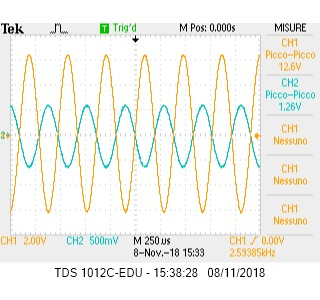
\includegraphics[scale=0.7]{foto1.jpg}
			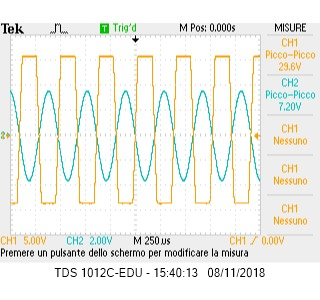
\includegraphics[scale=0.7]{foto2.jpg}
			\caption{screenshot dei segnali con e senza clipping}
			%\includegraphics[0.45\textwidth]{}
		\end{center}
		\caption{\small Ingresso (in alto) ed uscita (in basso) di un amplificatore invertente con OpAmp, in 
			zona lineare (a sinistra) e non (a destra)}
		\label{fig:oscinv}
	\end{figure}
	%
	
	Variando l'~ampiezza di $V_{in}$ si misura $V_{out}$ ed il relativo guadagno $A_V=V_{out}/V_{in}$ riportando i dati ottenuti in tabella~\ref{tab:guadagno} 
	e mostrandone un grafico in Fig. \ref{fit}. 
	Il fit è stato ottenuto mediante media pesata dei valori del guadagno; si può osservare come, alzando l'ampiezza, il guadagno diminuisca impercettibilmente. Trovandosi il tutto dentro una barra d'errore, non è considerabile un effetto significativo.
	L'incertezza sul guadagno è stato ottenuta sommando in quadratura le incertezze su Vin e Vout, dato che queste, essendo state misurate su canali diversi, si assumono scorrelate (anche l'incertezza sul digit è scorrelata).
	
	\begin{table}[h]
		\caption{$V_{out}$ in funzione di $V_{in}$ e relativo rapporto.}
		\label{tab:guadagno}
		\begin{center}
			\begin{tabular}{|c|c|c|}
				\hline
				$V_{in}$ (V) & $V_{out}$ (V)  & $A_V$ \\
				\hline
				\hline
				$ 0.50\pm 0.01 $ & $5.12 \pm 0.1 $ & $10.3 \pm 0.4 $ \\
				\hline
				$0.71 \pm 0.02 $ & $7.4 \pm 0.2 $ & $10.4 \pm 0.4 $ \\
				\hline
				$0.90 \pm 0.03 $ & $9.4 \pm 0.3 $ & $10.4 \pm 0.4 $ \\
				\hline
				$1.2 \pm 0.03 $ & $12.4 \pm 0.3 $ & $10.3 \pm 0.4 $ \\
				\hline
				$1.46 \pm 0.04 $ & $15.1 \pm 0.4 $ & $10.3 \pm 0.4 $ \\
				\hline
				$1.58 \pm 0.05 $ & $16.3 \pm 0.5 $ & $10.3 \pm 0.4 $ \\
				\hline
				$1.82 \pm 0.06 $ & $18.5 \pm 0.6 $ & $10.2 \pm 0.4 $ \\
				\hline
				$1.98 \pm 0.06 $ & $20.2 \pm 0.6 $ & $10.2 \pm 0.4 $ \\
				\hline
				$2.18 \pm 0.06 $ & $22.2 \pm 0.6 $ & $10.2 \pm 0.4 $ \\
				\hline
				$2.46 \pm 0.07 $ & $24.8 \pm 0.7 $ & $10.1 \pm 0.4 $ \\
				\hline
				$2.68 \pm 0.08 $ & $27.2 \pm 0.8 $ & $10.1 \pm 0.4 $ \\
				\hline
		
			\end{tabular}
		\end{center}
	\end{table}

		Gli ultimi 4 dati,riportati in tabella \ref{tab:daticlipping} sono stati presi per verificare il clipping, e quindi non considerati per il fit
		\begin{table}[h]
	
			\begin{center}
				\begin{tabular}{|c|c|c|}
					\hline
					$V_{in}$ (V) & $V_{out}$ (V)   \\
		\hline
		$2.96 \pm 0.09 $ & $28.8 \pm 0.8 $ \\
		\hline
		$3.04 \pm 0.09 $ & $29.3 \pm 0.8  $ \\
		\hline
		$3.20 \pm 0.09 $ & $29.4 \pm 0.9  $ \\
		\hline
		$3.25 \pm 0.1 $ & $29.5 \pm 0.9 $ \\
		\hline
		\end{tabular}
	\end{center}
\label{tab:daticlipping}
\caption{dati del segnale tagliato (clipping)}
\end{table}

	\begin{figure}\centering
			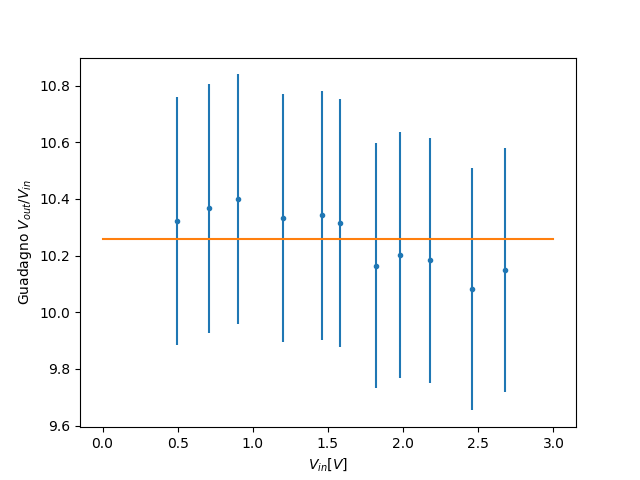
\includegraphics[scale=0.5]{fit.png}
				\caption{\small Linearit\`a dell'~amplificatore invertente}
			\label{fit}
	\end{figure}

	
	Si determina il guadagno mediante fit dei dati ottenuti:
	\[
	A_{best} = 10.258 \pm 0.001 \quad  \chi^2/ndof = 0.06
	\]

	Quindi gli errori sono stati sovrastimati.
	Cambiando la tensione dell'integrato si osserva clipping circa quando la tensione in uscita è pari a quella di alimentazione (in realtà un po' prima).
	
	%%%%%%%%%%%%%%%%%%
	%
	\section{Risposta in frequenza e \emph{slew rate}}
	\subsection{Risposta in frequenza del circuito}
	Si misura la risposta in frequenza del circuito, riportando i dati  in Tab. \ref{tab:bodeinv} e
	in un grafico di Bode in Fig. \ref{fig:bodeinv}, stimando la frequenza di taglio inferiore e 
	superiore \rem{indicare in che modo}.
	\[
	V_{in} = (\exn \pm \exn )\,\mathrm{V}
	\]
	\[
	f_L = (\exn \pm \exn )\,\mathrm{Hz}\;\;\;\;\;f_H = (\exn \pm \exn \;)\,\mathrm{kHz}
	\]
	\begin{table}[h]
		\caption{\small Guadagno dell'~amplificatore invertente in funzione della frequenza.}
		\label{tab:bodeinv}
		\begin{center}
			\begin{tabular}{|c|c|c|}	\hline
				$f_{in}$ (kHz) & $V_{out}$ (V) & $A$ (dB) \\
				\hline
				$\exn0.753 \pm \exn $ & $\exn10.4 \pm \exn $ & $\exn 1.01\pm \exn $\\
				\hline
				$\exn 1.76\pm \exn $ & $\exn 10.5\pm \exn $ & $\exn 1.01\pm \exn $\\
				\hline
				$\exn 2.90\pm \exn $ & $\exn 10.5\pm \exn $ & $\exn 1.01\pm \exn $\\
				\hline
				$\exn 6.22\pm \exn $ & $\exn 10.7\pm \exn $ & $\exn 1.01\pm \exn $\\
				\hline
				$\exn 12.2\pm \exn $ & $\exn 10.7\pm \exn $ & $\exn 1.00\pm \exn $\\
				\hline
				$\exn22.5 \pm \exn $ & $\exn 10.6\pm \exn $ & $\exn1.00\pm \exn $\\
				\hline
				$\exn44.9 \pm \exn $ & $\exn10.5 \pm \exn $ & $\exn 1.00\pm \exn $\\
				\hline
				$\exn 86.7\pm \exn $ & $\exn9.92 \pm \exn $ & $\exn 0.971 \pm \exn $\\
				\hline
				$\exn 166\pm \exn $ & $\exn8.48 \pm \exn $ & $\exn 0.903 \pm \exn $\\
				\hline
				$\exn 350\pm \exn $ & $\exn 4.02\pm \exn $ & $\exn0.714\pm \exn $\\
				\hline
				$\exn 435\pm \exn $ & $\exn 3\pm \exn $ & $\exn 0.639\pm \exn $\\
				\hline
				$\exn555 \pm \exn $ & $\exn2.44 \pm \exn $ & $\exn 0.545 \pm \exn $\\
				\hline
				$\exn 729\pm \exn $ & $\exn 2.22\pm \exn $ & $\exn 0.452 \pm \exn $\\
				\hline
				$\exn 1220\pm \exn $ & $\exn 1.38\pm \exn $ & $\exn 0.237\pm \exn $\\
				\hline
				$\exn212\pm \exn $ & $\exn4.96 \pm \exn $ & $\exn 0.858 \pm \exn $\\
				\hline
				$\exn251 \pm \exn $ & $\exn4.44 \pm \exn $ & $\exn 0.815\pm \exn $\\

				\hline
			\end{tabular}
		\end{center}
	\end{table} 
	
	
	
	\begin{figure}[h]
		\begin{center}
			
			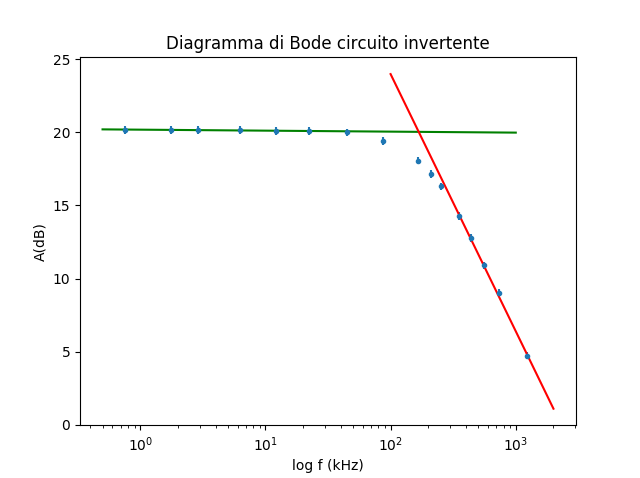
\includegraphics[width=0.7\textwidth]{bodeInvertente}
			\caption{\small Plot di Bode in ampiezza per l'~amplificatore invertente.}
			\label{fig:bodeinv}
		\end{center}
	\end{figure}
	%
	\subsection{Misura dello \emph{slew-rate}}
	Si misura direttamente lo \emph{slew-rate} dell'op-amp inviando in ingresso un'~onda quadra 
	di frequenza di $\sim 0.9$~kHz e di ampiezza $2.08$~V. Si ottiene:
	\[
	SR_\mathrm{misurato} = (12.5 \pm 0.5 )\,\mathrm{V/\mu s} \quad \mathrm{valore \; tipico}\, (13 )\,\mathrm{V/\mu s}\
	\]
Abbiamo misurato nel  punto a pendenza massima di $V_{out}$, che si trova proprio all'inizio dell'onda quadra, subito dopo la pendenza diminuisce di circa 0.5 $ \mathrm{V/\mu s}$

	%
	\section{Circuito integratore}
	Si monta il circuito integratore con i seguenti valori  dei componenti indicati: 
	\[
	R_1 = (0.997 \pm 0.008 \;) \,\mathrm{k}\Omega, \:\:\;\:\exn 
	R_2 = (9.92 \pm 0.08 \;) \,\mathrm{k}\Omega, \:\:\;\:\exn 
	C = (50.4 \pm 2.3 \;\;)\,\mathrm{nF}
	\]
	
	\subsection{Risposta in frequenza}
	
	Si invia un'~onda sinusoidale e si misura la risposta in frequenza dell'~amplificazione e della fase riportandoli 
	nella tabella \ref{tab:bodeinte} e in un diagramma di Bode in Fig. \ref{fig:bodeinte}. 
	\[
	V_{in} = (\exn \pm \exn )\,\mathrm{V}
	\]
	\rem{La fase pu\'o essere indicata in gradi, radianti, oppure come frazione $\phi/2\pi$}
	%
	\begin{table}[h]
		\caption{Guadagno e fase dell'~integratore invertente in funzione della frequenza.}
		\label{tab:bodeinte}
		\begin{center}
			\begin{tabular}{|c|c|c|c|c|}
				\hline
				$f_{in}$ (kHz) & $V_{out}$ (V) & $A$ (dB) & $\Delta t (\mu s)$ & $\phi$ \\
				\hline
				$\exn \pm \exn $ & $\exn \pm \exn $ & $\exn \pm \exn $ & $\exn \pm \exn $ & $\exn \pm \exn $ \\
				\hline
				$\exn \pm \exn $ & $\exn \pm \exn $ & $\exn \pm \exn $ & $\exn \pm \exn $ & $\exn \pm \exn $ \\
				\hline
				$\exn \pm \exn $ & $\exn \pm \exn $ & $\exn \pm \exn $ & $\exn \pm \exn $ & $\exn \pm \exn $ \\
				\hline
				$\exn \pm \exn $ & $\exn \pm \exn $ & $\exn \pm \exn $ & $\exn \pm \exn $ & $\exn \pm \exn $ \\
				\hline
				$\exn \pm \exn $ & $\exn \pm \exn $ & $\exn \pm \exn $ & $\exn \pm \exn $ & $\exn \pm \exn $ \\
				\hline
				$\exn \pm \exn $ & $\exn \pm \exn $ & $\exn \pm \exn $ & $\exn \pm \exn $ & $\exn \pm \exn $ \\
				\hline
				$\exn \pm \exn $ & $\exn \pm \exn $ & $\exn \pm \exn $ & $\exn \pm \exn $ & $\exn \pm \exn $ \\
				\hline
			\end{tabular}
		\end{center}
	\end{table} 
	%
	\begin{figure}[htb]
		\begin{center}
		
			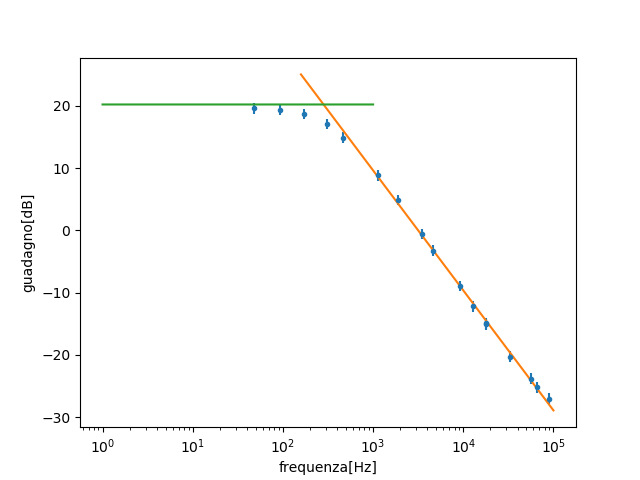
\includegraphics[0.45]{bodefrequenza.png}
			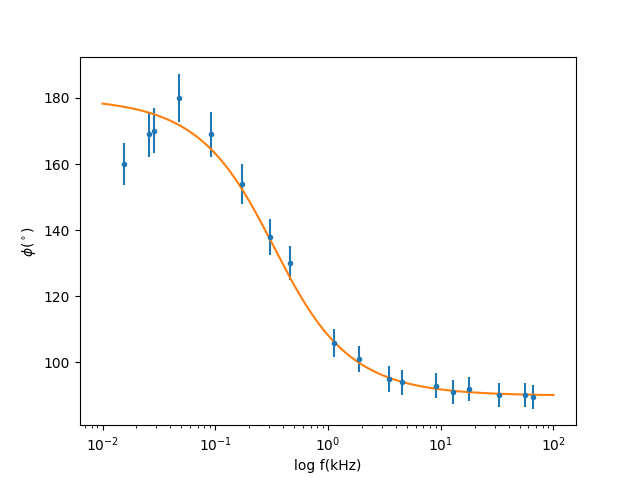
\includegraphics[0.45]{fase.png}
		\end{center}
		\caption{\small Plot di Bode in ampiezza (a sinistra) e fase (a destra) per il circuito integratore.}
		\label{fig:bodeinte}
	\end{figure}
	%
	
	Si ricava una stima delle caratteristiche principali dell'andamento (guadagno a bassa frequenza, frequenza di taglio, e pendenza ad alta frequenza)
	e si confrontano con quanto atteso. Non si effettua la stima degli errori, trattandosi di misure qualitative.
	
	\rem{Indicare brevemente come sono stati ottenuti i valori attesi}
	
	\begin{align*}
	A_M &= (\exn )\,\mathrm{dB} & \mathrm{atteso} &:\,(\exn  )\, \mathrm{dB}  \\
	f_H &= (\exn )\,\mathrm{Hz} & \mathrm{atteso} &:\,(\exn  )\, \mathrm{Hz} \\
	{\mathrm{d}A_V}/{\mathrm{d}f} &= (\exn )\,\mathrm{dB/decade} & \mathrm{atteso} &:\,(\exn  )\, \mathrm{dB/decade}  \\
	\end{align*}
	
	
	%
	\subsection*{Risposta ad un'~onda quadra}
	Si invia all'~ingresso un'~onda quadra di frequenza $\sim xxx\,kHz$ e ampiezza $\sim xxx\,V$.
	Si riporta in Fig. \ref{fig:oscinte} le forme d'~onda acquisite all'~oscillografo per l'~ingresso
	e l'~uscita. 
	
	\rem{Commentare se che il circuito si comporta come un integratore.}
	%
	\begin{figure}[htb]
		\begin{center}
			\framebox(200,200){Inserire screenshot oscillografo per integratore}
			%\includegraphics[0.45\textwidth]{}
		\end{center}
		\caption{\small Ingresso (in alto) ed uscita (in basso) del circuito integratore per un'~onda quadra.}
		\label{fig:oscinte}
	\end{figure}
	%
	
	Si misura l'~ampiezza dell'~onda  in uscita e si confronta il valore atteso.
	
	\rem{Indicare brevemente come sono stati ottenuti i valori attesi}
	\begin{align*}
	V_{out} &= (\exn )\,\mathrm{V} & \mathrm{atteso} &:\,(\exn  )\, \mathrm{V}  \\
	\end{align*}
	
	\rem{Inserire commento sulla dipendenza dell'~uscita dalla frequenza.}
	%
	
	\subsection{Discussione}
	
	\rem{Inserire commenti su quanto osservato ed eventuali deviazioni. 
		In particolare: attenuazione ad alte frequenze, dipendenza della fase dalla frequenza, funzione di $R_2$. }
	
	%%%%%%%%%%%%%%%%%%%%%%%%
	
\end{document}          
